% 2-page report (AI Assignment 2: Real-Life Use Cases of RL, Mini Project).
% Numbers come from numbers.tex (generated by scripts/make_figures.py from results/) unless a
% comment names another source file. Figures: ../figures (fig_psi.png from scripts/make_fig_psi.py).
% Build from report/: pdflatex report (twice).
\documentclass[10pt,twocolumn,a4paper]{article}
\usepackage[margin=1.35cm,top=1.1cm,bottom=1.4cm,columnsep=0.55cm]{geometry}
\usepackage[T1]{fontenc}
\usepackage{lmodern,microtype,amsmath,amssymb,graphicx,booktabs,xcolor,array}
\usepackage[hidelinks]{hyperref}
\usepackage[capitalise,nameinlink]{cleveref}
\crefname{table}{Tab.}{Tabs.}\crefname{figure}{Fig.}{Figs.}
\usepackage{titlesec,enumitem,caption,subcaption}
\titleformat{\section}{\normalsize\bfseries}{\thesection}{0.5em}{}
\titlespacing*{\section}{0pt}{4pt}{2pt}
\titleformat{\paragraph}[runin]{\normalsize\bfseries}{}{0pt}{}
\titlespacing*{\paragraph}{0pt}{2pt}{0.6em}
\setlist{nosep,leftmargin=1.1em}
\captionsetup{font=footnotesize,labelfont=bf,skip=2pt}
\setlength{\textfloatsep}{5pt}\setlength{\floatsep}{4pt}\setlength{\dbltextfloatsep}{5pt}
\setlength{\abovedisplayskip}{2pt}\setlength{\belowdisplayskip}{2pt}
\newcommand{\repo}{https://github.com/bot2048/cabinet-bargaining-marl}
\newcommand{\code}[1]{\href{\repo/blob/main/#1}{\texttt{\footnotesize #1}}}
% generated by scripts/make_figures.py -- do not edit
\newcommand{\AfDemFormHi}{0.51}
\newcommand{\AfDemFormLo}{0.44}
\newcommand{\AfDemMaxDev}{0.02}
\newcommand{\AfDemSeeds}{3}
\newcommand{\AfDemSlope}{\ensuremath{-}0.02 to +0.12}
\newcommand{\AfPropFormHi}{0.73}
\newcommand{\AfPropFormLo}{0.65}
\newcommand{\AfPropMaxDev}{0.23}
\newcommand{\AfPropSeeds}{3}
\newcommand{\AfPropSlope}{+0.38 to +0.75}
\newcommand{\AtDemDummy}{0.0\%}
\newcommand{\AtDemFormHi}{0.47}
\newcommand{\AtDemFormLo}{0.39}
\newcommand{\AtDemMaxDev}{0.03}
\newcommand{\AtDemSeeds}{3}
\newcommand{\AtDemSlope}{+0.06 to +0.28}
\newcommand{\AtPropBigHi}{0.71}
\newcommand{\AtPropBigLo}{0.65}
\newcommand{\AtPropDumHi}{0.39}
\newcommand{\AtPropDumLo}{0.36}
\newcommand{\AtPropDummy}{5.4\%}
\newcommand{\AtPropFormHi}{0.71}
\newcommand{\AtPropFormLo}{0.36}
\newcommand{\AtPropMaxDev}{0.20}
\newcommand{\AtPropSeeds}{3}
\newcommand{\AtPropSlope}{\ensuremath{-}0.12 to +1.63}
\newcommand{\BaseBeta}{+0.468}
\newcommand{\BaseCollapse}{+0.000}
\newcommand{\BaseDg}{+0.132}
\newcommand{\BaseFail}{+0.039}
\newcommand{\BaseGamma}{+0.249}
\newcommand{\BaseGlead}{--}
\newcommand{\BaseGnu}{--}
\newcommand{\BasePhi}{+0.146}
\newcommand{\BasePhiNu}{+0.147}
\newcommand{\BaseRtwo}{0.77}
\newcommand{\BaseRtwoBz}{0.85}
\newcommand{\BaseSeeds}{5}
\newcommand{\BfBigForm}{0.71}
\newcommand{\BfDummyForm}{0.41}
\newcommand{\BrGainFive}{0.056}
\newcommand{\BrGainSeven}{0.153}
\newcommand{\BrGainThree}{0.013}
\newcommand{\BrSeatGain}{0.007}
\newcommand{\BrSevenXbest}{0.073}
\newcommand{\BrSevenXlearned}{0.133}
\newcommand{\CmAcross}{+0.0004}
\newcommand{\CmSame}{+0.0020}
\newcommand{\DemA}{+0.096}
\newcommand{\DemB}{0.81}
\newcommand{\DemClose}{\ensuremath{-}0.023}
\newcommand{\DemFirst}{+0.026}
\newcommand{\DemG}{\ensuremath{-}0.039}
\newcommand{\DemRtwo}{0.76}
\newcommand{\DemSeeds}{10}
\newcommand{\DmaePrivLo}{+0.016}
\newcommand{\EntHigh}{+0.121}
\newcommand{\EntLow}{+0.138}
\newcommand{\EntMid}{+0.124}
\newcommand{\EoneAbsGap}{0.085}
\newcommand{\EoneGap}{\ensuremath{-}0.074}
\newcommand{\EstarBeta}{+0.426}
\newcommand{\EstarCollapse}{+0.151}
\newcommand{\EstarDg}{+0.093}
\newcommand{\EstarFail}{+0.046}
\newcommand{\EstarGamma}{+0.052}
\newcommand{\EstarGlead}{+0.156}
\newcommand{\EstarGnu}{+0.205}
\newcommand{\EstarPhi}{\ensuremath{-}0.008}
\newcommand{\EstarPhiNu}{+0.143}
\newcommand{\EstarRtwo}{0.44}
\newcommand{\EstarRtwoBz}{0.55}
\newcommand{\EstarSeeds}{10}
\newcommand{\ExpDemB}{0.82--0.86}
\newcommand{\ExpDemG}{\ensuremath{-}0.009 to +0.003}
\newcommand{\ExpDemSeeds}{3}
\newcommand{\ExploreB}{1.05}
\newcommand{\ExploreClose}{\ensuremath{-}0.025}
\newcommand{\ExploreCloserFive}{0.34}
\newcommand{\ExploreCloserThree}{0.44}
\newcommand{\ExploreFirst}{+0.035}
\newcommand{\EzeroAbsGap}{0.017}
\newcommand{\EzeroCellsOK}{6}
\newcommand{\EzeroFail}{2.2\%}
\newcommand{\EzeroGap}{+0.001}
\newcommand{\EzeroSeeds}{10}
\newcommand{\FspBeta}{+0.414}
\newcommand{\FspCollapse}{+0.166}
\newcommand{\FspDg}{+0.094}
\newcommand{\FspFail}{+0.029}
\newcommand{\FspGamma}{+0.065}
\newcommand{\FspGlead}{+0.153}
\newcommand{\FspGnu}{+0.219}
\newcommand{\FspPhi}{+0.001}
\newcommand{\FspPhiNu}{+0.152}
\newcommand{\FspRtwo}{0.42}
\newcommand{\FspRtwoBz}{0.52}
\newcommand{\FspSeeds}{3}
\newcommand{\GainBASE}{+0.017}
\newcommand{\GainBASEGamson}{+0.008}
\newcommand{\GainBASEMax}{+0.023}
\newcommand{\GainBASEMyopic}{\ensuremath{-}0.004}
\newcommand{\GainDemRel}{19\%}
\newcommand{\GainDemand}{+0.14}
\newcommand{\GainEstar}{+0.016}
\newcommand{\GainEstarGamson}{+0.020}
\newcommand{\GainEstarMax}{+0.024}
\newcommand{\GainEstarMyopic}{+0.076}
\newcommand{\GainEzero}{0.040}
\newcommand{\GainEzeroGamson}{0.019}
\newcommand{\GainEzeroMyopic}{0.037}
\newcommand{\GainEzeroRel}{20\%}
\newcommand{\GainLong}{+0.015}
\newcommand{\GainLongGamson}{+0.037}
\newcommand{\GainLongMyopic}{+0.088}
\newcommand{\GainLongRel}{10\%}
\newcommand{\GainMappo}{+0.018}
\newcommand{\GainPropRel}{18\%}
\newcommand{\GcBF}{0.42}
\newcommand{\GcPrivHi}{0.19}
\newcommand{\GcPrivLo}{0.12}
\newcommand{\GcPubHi}{0.53}
\newcommand{\GcPubLo}{0.41}
\newcommand{\HoneDiff}{0.34}
\newcommand{\HoneHi}{0.36}
\newcommand{\HoneLo}{0.32}
\newcommand{\HoneP}{5\times10^{\ensuremath{-}6}}
\newcommand{\HthreeHi}{\ensuremath{-}0.030}
\newcommand{\HthreeLo}{\ensuremath{-}0.047}
\newcommand{\HthreeMean}{\ensuremath{-}0.039}
\newcommand{\HtwoDiff}{0.36}
\newcommand{\HtwoHi}{0.37}
\newcommand{\HtwoLo}{0.34}
\newcommand{\KeyCount}{0.573}
\newcommand{\KeyDiff}{+0.015}
\newcommand{\KeyDiffHi}{+0.056}
\newcommand{\KeyDiffLo}{\ensuremath{-}0.021}
\newcommand{\KeyN}{131}
\newcommand{\KeySeat}{0.598}
\newcommand{\KeyShare}{0.589}
\newcommand{\LamzeroBeta}{+0.445}
\newcommand{\LamzeroCollapse}{+0.092}
\newcommand{\LamzeroDg}{+0.096}
\newcommand{\LamzeroFail}{+0.081}
\newcommand{\LamzeroGamma}{\ensuremath{-}0.006}
\newcommand{\LamzeroGlead}{+0.069}
\newcommand{\LamzeroGnu}{+0.142}
\newcommand{\LamzeroPhi}{\ensuremath{-}0.040}
\newcommand{\LamzeroPhiNu}{+0.113}
\newcommand{\LamzeroRtwo}{0.34}
\newcommand{\LamzeroRtwoBz}{0.55}
\newcommand{\LamzeroSeeds}{3}
\newcommand{\LockinB}{1.28}
\newcommand{\LockinClose}{\ensuremath{-}0.269}
\newcommand{\LockinCloserFive}{0.16}
\newcommand{\LockinCloserThree}{0.35}
\newcommand{\LockinFirst}{+0.009}
\newcommand{\LocoHi}{+0.013}
\newcommand{\LocoLo}{\ensuremath{-}0.004}
\newcommand{\LongBaseG}{+0.295}
\newcommand{\LongBaseGlead}{--}
\newcommand{\LongBaseGnu}{--}
\newcommand{\LongBasePhiNu}{+0.182}
\newcommand{\LongEstarG}{+0.088}
\newcommand{\LongEstarGlead}{+0.158}
\newcommand{\LongEstarGnu}{+0.240}
\newcommand{\LongEstarPhiNu}{+0.151}
\newcommand{\LongMfourG}{\ensuremath{-}0.004}
\newcommand{\LongMfourGlead}{\ensuremath{-}0.028}
\newcommand{\LongMfourGnu}{+0.139}
\newcommand{\LongMfourPhiNu}{+0.170}
\newcommand{\LongMnineG}{+0.007}
\newcommand{\LongMnineGlead}{+0.770}
\newcommand{\LongMnineGnu}{+0.007}
\newcommand{\LongMninePhiNu}{+0.021}
\newcommand{\LooMeightBeta}{+0.399}
\newcommand{\LooMeightCollapse}{+0.000}
\newcommand{\LooMeightDg}{+0.097}
\newcommand{\LooMeightFail}{+0.083}
\newcommand{\LooMeightGamma}{+0.207}
\newcommand{\LooMeightPhi}{+0.061}
\newcommand{\LooMeightPhiNu}{+0.196}
\newcommand{\LooMeightRtwo}{0.71}
\newcommand{\LooMeightRtwoBz}{0.75}
\newcommand{\LooMeightSeeds}{3}
\newcommand{\LooMfiveBeta}{+0.429}
\newcommand{\LooMfiveCollapse}{+0.147}
\newcommand{\LooMfiveDg}{+0.090}
\newcommand{\LooMfiveFail}{+0.029}
\newcommand{\LooMfiveGamma}{+0.210}
\newcommand{\LooMfivePhi}{+0.073}
\newcommand{\LooMfivePhiNu}{+0.073}
\newcommand{\LooMfiveRtwo}{0.78}
\newcommand{\LooMfiveRtwoBz}{0.83}
\newcommand{\LooMfiveSeeds}{3}
\newcommand{\LooMfourBeta}{+0.394}
\newcommand{\LooMfourCollapse}{+0.079}
\newcommand{\LooMfourDg}{+0.108}
\newcommand{\LooMfourFail}{+0.038}
\newcommand{\LooMfourGamma}{+0.221}
\newcommand{\LooMfourPhi}{+0.084}
\newcommand{\LooMfourPhiNu}{+0.177}
\newcommand{\LooMfourRtwo}{0.67}
\newcommand{\LooMfourRtwoBz}{0.69}
\newcommand{\LooMfourSeeds}{3}
\newcommand{\LooMnineBeta}{+0.413}
\newcommand{\LooMnineCollapse}{+0.136}
\newcommand{\LooMnineDg}{+0.093}
\newcommand{\LooMnineFail}{+0.040}
\newcommand{\LooMnineGamma}{+0.053}
\newcommand{\LooMninePhi}{\ensuremath{-}0.009}
\newcommand{\LooMninePhiNu}{+0.147}
\newcommand{\LooMnineRtwo}{0.41}
\newcommand{\LooMnineRtwoBz}{0.51}
\newcommand{\LooMnineSeeds}{3}
\newcommand{\LooMoneBeta}{+0.460}
\newcommand{\LooMoneCollapse}{+0.053}
\newcommand{\LooMoneDg}{+0.098}
\newcommand{\LooMoneFail}{+0.074}
\newcommand{\LooMoneGamma}{\ensuremath{-}0.040}
\newcommand{\LooMonePhi}{\ensuremath{-}0.060}
\newcommand{\LooMonePhiNu}{+0.094}
\newcommand{\LooMoneRtwo}{0.38}
\newcommand{\LooMoneRtwoBz}{0.57}
\newcommand{\LooMoneSeeds}{3}
\newcommand{\LooMtenBeta}{+0.356}
\newcommand{\LooMtenCollapse}{+0.151}
\newcommand{\LooMtenDg}{+0.116}
\newcommand{\LooMtenFail}{+0.047}
\newcommand{\LooMtenGamma}{+0.092}
\newcommand{\LooMtenPhi}{+0.071}
\newcommand{\LooMtenPhiNu}{+0.226}
\newcommand{\LooMtenRtwo}{0.37}
\newcommand{\LooMtenRtwoBz}{0.46}
\newcommand{\LooMtenSeeds}{3}
\newcommand{\MaeBF}{0.144}
\newcommand{\MaeGamson}{0.052}
\newcommand{\MaePrivHi}{0.090}
\newcommand{\MaePrivLo}{0.087}
\newcommand{\MaePubHi}{0.167}
\newcommand{\MaePubLo}{0.130}
\newcommand{\MappoBeta}{+0.457}
\newcommand{\MappoCollapse}{+0.128}
\newcommand{\MappoDg}{+0.085}
\newcommand{\MappoFail}{+0.053}
\newcommand{\MappoGamma}{+0.037}
\newcommand{\MappoGlead}{+0.124}
\newcommand{\MappoGnu}{+0.188}
\newcommand{\MappoPhi}{\ensuremath{-}0.013}
\newcommand{\MappoPhiNu}{+0.139}
\newcommand{\MappoRtwo}{0.45}
\newcommand{\MappoRtwoBz}{0.52}
\newcommand{\MappoSeeds}{10}
\newcommand{\MeightBeta}{+0.356}
\newcommand{\MeightCollapse}{+0.006}
\newcommand{\MeightDg}{+0.138}
\newcommand{\MeightFail}{+0.035}
\newcommand{\MeightGamma}{+0.223}
\newcommand{\MeightPhi}{+0.132}
\newcommand{\MeightPhiNu}{+0.132}
\newcommand{\MeightRtwo}{0.70}
\newcommand{\MeightRtwoBz}{0.83}
\newcommand{\MeightSeeds}{3}
\newcommand{\MfiveBeta}{+0.364}
\newcommand{\MfiveCollapse}{+0.000}
\newcommand{\MfiveDg}{+0.149}
\newcommand{\MfiveFail}{+0.074}
\newcommand{\MfiveGamma}{+0.172}
\newcommand{\MfiveGlead}{+0.227}
\newcommand{\MfiveGnu}{+0.131}
\newcommand{\MfivePhi}{+0.111}
\newcommand{\MfivePhiNu}{+0.205}
\newcommand{\MfiveRtwo}{0.40}
\newcommand{\MfiveRtwoBz}{0.54}
\newcommand{\MfiveSeeds}{3}
\newcommand{\MfourBeta}{+0.493}
\newcommand{\MfourCollapse}{+0.000}
\newcommand{\MfourDg}{+0.072}
\newcommand{\MfourFail}{+0.122}
\newcommand{\MfourGamma}{\ensuremath{-}0.036}
\newcommand{\MfourGlead}{\ensuremath{-}0.032}
\newcommand{\MfourGnu}{+0.107}
\newcommand{\MfourPhi}{\ensuremath{-}0.010}
\newcommand{\MfourPhiNu}{+0.157}
\newcommand{\MfourRtwo}{0.50}
\newcommand{\MfourRtwoBz}{0.63}
\newcommand{\MfourSeeds}{5}
\newcommand{\MnineBeta}{+0.457}
\newcommand{\MnineCollapse}{+0.000}
\newcommand{\MnineDg}{+0.089}
\newcommand{\MnineFail}{+0.060}
\newcommand{\MnineGamma}{\ensuremath{-}0.029}
\newcommand{\MnineGlead}{+0.803}
\newcommand{\MnineGnu}{\ensuremath{-}0.029}
\newcommand{\MninePhi}{\ensuremath{-}0.005}
\newcommand{\MninePhiNu}{\ensuremath{-}0.006}
\newcommand{\MnineRtwo}{0.41}
\newcommand{\MnineRtwoBz}{0.53}
\newcommand{\MnineSeeds}{5}
\newcommand{\MoneBeta}{+0.379}
\newcommand{\MoneCollapse}{+0.000}
\newcommand{\MoneDg}{+0.154}
\newcommand{\MoneFail}{+0.027}
\newcommand{\MoneGamma}{+0.291}
\newcommand{\MonePhi}{+0.173}
\newcommand{\MonePhiNu}{+0.174}
\newcommand{\MoneRtwo}{0.82}
\newcommand{\MoneRtwoBz}{0.90}
\newcommand{\MoneSeeds}{3}
\newcommand{\MpatientBeta}{+0.249}
\newcommand{\MpatientCollapse}{+0.000}
\newcommand{\MpatientDg}{+0.182}
\newcommand{\MpatientFail}{+0.083}
\newcommand{\MpatientGamma}{+0.320}
\newcommand{\MpatientPhi}{+0.192}
\newcommand{\MpatientPhiNu}{+0.192}
\newcommand{\MpatientRtwo}{0.79}
\newcommand{\MpatientRtwoBz}{0.80}
\newcommand{\MpatientSeeds}{3}
\newcommand{\MpatientrecBeta}{+0.256}
\newcommand{\MpatientrecCollapse}{+0.000}
\newcommand{\MpatientrecDg}{+0.178}
\newcommand{\MpatientrecFail}{+0.101}
\newcommand{\MpatientrecGamma}{+0.295}
\newcommand{\MpatientrecPhi}{+0.185}
\newcommand{\MpatientrecPhiNu}{+0.185}
\newcommand{\MpatientrecRtwo}{0.72}
\newcommand{\MpatientrecRtwoBz}{0.73}
\newcommand{\MpatientrecSeeds}{3}
\newcommand{\MtenBeta}{+0.340}
\newcommand{\MtenCollapse}{+0.000}
\newcommand{\MtenDg}{+0.098}
\newcommand{\MtenFail}{+0.028}
\newcommand{\MtenGamma}{+0.159}
\newcommand{\MtenPhi}{+0.027}
\newcommand{\MtenPhiNu}{+0.028}
\newcommand{\MtenRtwo}{0.61}
\newcommand{\MtenRtwoBz}{0.73}
\newcommand{\MtenSeeds}{5}
\newcommand{\MtwelveBeta}{+0.416}
\newcommand{\MtwelveCollapse}{+0.116}
\newcommand{\MtwelveDg}{+0.122}
\newcommand{\MtwelveFail}{+0.053}
\newcommand{\MtwelveGamma}{\ensuremath{-}0.059}
\newcommand{\MtwelveGlead}{+0.548}
\newcommand{\MtwelveGnu}{+0.147}
\newcommand{\MtwelvePhi}{\ensuremath{-}0.066}
\newcommand{\MtwelvePhiNu}{+0.141}
\newcommand{\MtwelveRtwo}{0.34}
\newcommand{\MtwelveRtwoBz}{0.52}
\newcommand{\MtwelveSeeds}{3}
\newcommand{\NprotSeeds}{10}
\newcommand{\OwnDemA}{0.06--0.13}
\newcommand{\OwnDemB}{0.74--0.87}
\newcommand{\OwnDemBbz}{0.70--0.86}
\newcommand{\OwnDemG}{\ensuremath{-}0.07 to \ensuremath{-}0.01}
\newcommand{\OwnDemGbz}{\ensuremath{-}0.08 to \ensuremath{-}0.02}
\newcommand{\OwnDemGnu}{\ensuremath{-}0.07 to \ensuremath{-}0.01}
\newcommand{\OwnDemMatch}{11\%--14\%}
\newcommand{\OwnDemMatchB}{0.68--0.83}
\newcommand{\OwnDemMatchBbz}{0.68--0.89}
\newcommand{\OwnDemMatchG}{\ensuremath{-}0.09 to \ensuremath{-}0.04}
\newcommand{\OwnDemPhiNu}{\ensuremath{-}0.04 to \ensuremath{-}0.01}
\newcommand{\OwnDemRtwo}{0.80--0.89}
\newcommand{\OwnDemSeeds}{10}
\newcommand{\OwnExpB}{0.86--0.87}
\newcommand{\OwnExpG}{\ensuremath{-}0.02 to 0.00}
\newcommand{\OwnExpGbz}{\ensuremath{-}0.03 to 0.00}
\newcommand{\OwnExpRtwo}{0.86--0.87}
\newcommand{\OwnPropA}{0.05--0.09}
\newcommand{\OwnPropB}{0.49--0.55}
\newcommand{\OwnPropBbz}{0.48--0.55}
\newcommand{\OwnPropG}{+0.21--0.34}
\newcommand{\OwnPropGbz}{+0.24--0.38}
\newcommand{\OwnPropGnu}{+0.21--0.34}
\newcommand{\OwnPropMatch}{7\%--9\%}
\newcommand{\OwnPropMatchB}{0.43--0.60}
\newcommand{\OwnPropMatchBbz}{0.51--0.65}
\newcommand{\OwnPropMatchG}{+0.19--0.30}
\newcommand{\OwnPropPhiNu}{+0.08--0.17}
\newcommand{\OwnPropRtwo}{0.84--0.94}
\newcommand{\OwnPropSeeds}{10}
\newcommand{\OwnWideA}{0.11--0.12}
\newcommand{\OwnWideB}{0.63--0.67}
\newcommand{\OwnWideBbz}{0.57--0.63}
\newcommand{\OwnWideG}{+0.01--0.08}
\newcommand{\OwnWideGbz}{+0.05--0.11}
\newcommand{\OwnWideGnu}{+0.15--0.22}
\newcommand{\OwnWideMatch}{11\%--12\%}
\newcommand{\OwnWideMatchB}{0.52--0.58}
\newcommand{\OwnWideMatchBbz}{0.53--0.61}
\newcommand{\OwnWideMatchG}{\ensuremath{-}0.01 to +0.09}
\newcommand{\OwnWidePhiNu}{+0.14--0.18}
\newcommand{\OwnWideRtwo}{0.71--0.73}
\newcommand{\OwnWideSeeds}{3}
\newcommand{\PgAllIdeology}{31.9\%}
\newcommand{\PgAllLearned}{19.7\%}
\newcommand{\PgAllN}{441}
\newcommand{\PgAllRandom}{18.9\%}
\newcommand{\PgAllRiker}{20.4\%}
\newcommand{\PgBeta}{+0.548}
\newcommand{\PgGamma}{+0.050}
\newcommand{\PgIdeoLearned}{22.3\%}
\newcommand{\PgIdeology}{31.7\%}
\newcommand{\PgLearned}{21.7\%}
\newcommand{\PgPhi}{\ensuremath{-}0.034}
\newcommand{\PgPhiNu}{+0.112}
\newcommand{\PgRandom}{21.7\%}
\newcommand{\PgRiker}{19.7\%}
\newcommand{\PgRtwo}{0.64}
\newcommand{\PgRtwoBz}{0.73}
\newcommand{\PoneHi}{+0.24}
\newcommand{\PoneLo}{\ensuremath{-}0.12}
\newcommand{\PropA}{+0.087}
\newcommand{\PropB}{0.45}
\newcommand{\PropClose}{--}
\newcommand{\PropFirst}{--}
\newcommand{\PropG}{+0.304}
\newcommand{\PropRtwo}{0.89}
\newcommand{\PropSeeds}{10}
\newcommand{\PsiAfDemEx}{+0.289}
\newcommand{\PsiAfDemReg}{--}
\newcommand{\PsiAfProp}{+0.367}
\newcommand{\PsiAfPropAll}{+0.366}
\newcommand{\PsiAfPropCov}{0.84}
\newcommand{\PsiAfPropEx}{+0.508}
\newcommand{\PsiAfPropExit}{+0.000}
\newcommand{\PsiAfPropNu}{+0.000}
\newcommand{\PsiAfPropPol}{+0.000}
\newcommand{\PsiAfPropReg}{formateur}
\newcommand{\PsiAfPropSe}{0.046}
\newcommand{\PsiAfPropSig}{+0.367}
\newcommand{\PsiBase}{+0.229}
\newcommand{\PsiBaseAll}{+0.222}
\newcommand{\PsiBaseCov}{0.73}
\newcommand{\PsiBaseEx}{+0.389}
\newcommand{\PsiBaseExit}{+0.000}
\newcommand{\PsiBaseNu}{+0.000}
\newcommand{\PsiBasePol}{+0.000}
\newcommand{\PsiBaseReg}{formateur}
\newcommand{\PsiBaseSe}{0.021}
\newcommand{\PsiBaseSig}{+0.229}
\newcommand{\PsiCovHi}{0.89}
\newcommand{\PsiCovLo}{0.70}
\newcommand{\PsiEntHi}{+0.169}
\newcommand{\PsiEntHiAll}{+0.163}
\newcommand{\PsiEntHiCov}{0.73}
\newcommand{\PsiEntHiEx}{+0.318}
\newcommand{\PsiEntHiExit}{+0.000}
\newcommand{\PsiEntHiNu}{+0.000}
\newcommand{\PsiEntHiPol}{+0.000}
\newcommand{\PsiEntHiReg}{formateur}
\newcommand{\PsiEntHiSe}{0.015}
\newcommand{\PsiEntHiSig}{+0.169}
\newcommand{\PsiEntLo}{+0.220}
\newcommand{\PsiEntLoAll}{+0.219}
\newcommand{\PsiEntLoCov}{0.70}
\newcommand{\PsiEntLoEx}{+0.394}
\newcommand{\PsiEntLoExit}{+0.000}
\newcommand{\PsiEntLoNu}{+0.000}
\newcommand{\PsiEntLoPol}{+0.000}
\newcommand{\PsiEntLoReg}{formateur}
\newcommand{\PsiEntLoSe}{0.019}
\newcommand{\PsiEntLoSig}{+0.220}
\newcommand{\PsiEntMd}{+0.180}
\newcommand{\PsiEntMdAll}{+0.182}
\newcommand{\PsiEntMdCov}{0.74}
\newcommand{\PsiEntMdEx}{+0.356}
\newcommand{\PsiEntMdExit}{+0.000}
\newcommand{\PsiEntMdNu}{+0.000}
\newcommand{\PsiEntMdPol}{+0.000}
\newcommand{\PsiEntMdReg}{formateur}
\newcommand{\PsiEntMdSe}{0.034}
\newcommand{\PsiEntMdSig}{+0.180}
\newcommand{\PsiEone}{+0.284}
\newcommand{\PsiEoneAll}{+0.278}
\newcommand{\PsiEoneCov}{0.77}
\newcommand{\PsiEoneEx}{+0.447}
\newcommand{\PsiEoneExit}{+0.000}
\newcommand{\PsiEoneNu}{+0.000}
\newcommand{\PsiEonePol}{+0.000}
\newcommand{\PsiEoneReg}{formateur}
\newcommand{\PsiEoneSe}{0.017}
\newcommand{\PsiEoneSig}{+0.284}
\newcommand{\PsiEstar}{+0.164}
\newcommand{\PsiEstarAll}{+0.159}
\newcommand{\PsiEstarCov}{0.87}
\newcommand{\PsiEstarEx}{+0.379}
\newcommand{\PsiEstarExit}{\ensuremath{-}0.001}
\newcommand{\PsiEstarNu}{+0.114}
\newcommand{\PsiEstarPol}{+0.016}
\newcommand{\PsiEstarReg}{formateur}
\newcommand{\PsiEstarSe}{0.009}
\newcommand{\PsiEstarSig}{+0.036}
\newcommand{\PsiExpDemEx}{+0.147}
\newcommand{\PsiExpDemReg}{--}
\newcommand{\PsiEzeroAbsGap}{0.017}
\newcommand{\PsiEzeroCells}{6}
\newcommand{\PsiEzeroFiveNine}{0.481}
\newcommand{\PsiEzeroFiveNineBF}{0.460}
\newcommand{\PsiEzeroSevenEight}{0.468}
\newcommand{\PsiEzeroSevenEightBF}{0.543}
\newcommand{\PsiEzeroThreeNine}{0.400}
\newcommand{\PsiEzeroThreeNineBF}{0.400}
\newcommand{\PsiFsp}{+0.181}
\newcommand{\PsiFspAll}{+0.176}
\newcommand{\PsiFspCov}{0.86}
\newcommand{\PsiFspEx}{+0.395}
\newcommand{\PsiFspExit}{\ensuremath{-}0.001}
\newcommand{\PsiFspNu}{+0.117}
\newcommand{\PsiFspPol}{+0.017}
\newcommand{\PsiFspReg}{formateur}
\newcommand{\PsiFspSe}{0.021}
\newcommand{\PsiFspSig}{+0.049}
\newcommand{\PsiLongBase}{+0.264}
\newcommand{\PsiLongBaseAll}{+0.258}
\newcommand{\PsiLongBaseCov}{0.71}
\newcommand{\PsiLongBaseEx}{+0.441}
\newcommand{\PsiLongBaseExit}{+0.000}
\newcommand{\PsiLongBaseNu}{+0.000}
\newcommand{\PsiLongBasePol}{+0.000}
\newcommand{\PsiLongBaseReg}{formateur}
\newcommand{\PsiLongBaseSe}{0.003}
\newcommand{\PsiLongBaseSig}{+0.264}
\newcommand{\PsiLongEstar}{+0.234}
\newcommand{\PsiLongEstarAll}{+0.222}
\newcommand{\PsiLongEstarCov}{0.82}
\newcommand{\PsiLongEstarEx}{+0.442}
\newcommand{\PsiLongEstarExit}{\ensuremath{-}0.002}
\newcommand{\PsiLongEstarNu}{+0.119}
\newcommand{\PsiLongEstarPol}{+0.023}
\newcommand{\PsiLongEstarReg}{formateur}
\newcommand{\PsiLongEstarSe}{0.027}
\newcommand{\PsiLongEstarSig}{+0.093}
\newcommand{\PsiLongMfour}{+0.106}
\newcommand{\PsiLongMfourAll}{+0.107}
\newcommand{\PsiLongMfourCov}{0.70}
\newcommand{\PsiLongMfourEx}{+0.312}
\newcommand{\PsiLongMfourExit}{+0.000}
\newcommand{\PsiLongMfourNu}{+0.118}
\newcommand{\PsiLongMfourPol}{+0.000}
\newcommand{\PsiLongMfourReg}{formateur}
\newcommand{\PsiLongMfourSe}{0.006}
\newcommand{\PsiLongMfourSig}{\ensuremath{-}0.012}
\newcommand{\PsiLongMnine}{+0.107}
\newcommand{\PsiLongMnineAll}{+0.099}
\newcommand{\PsiLongMnineCov}{0.77}
\newcommand{\PsiLongMnineEx}{+0.323}
\newcommand{\PsiLongMnineExit}{+0.000}
\newcommand{\PsiLongMnineNu}{+0.000}
\newcommand{\PsiLongMninePol}{+0.091}
\newcommand{\PsiLongMnineReg}{formateur}
\newcommand{\PsiLongMnineSe}{0.002}
\newcommand{\PsiLongMnineSig}{+0.016}
\newcommand{\PsiLooMeight}{+0.355}
\newcommand{\PsiLooMeightAll}{+0.344}
\newcommand{\PsiLooMeightCov}{0.86}
\newcommand{\PsiLooMeightEx}{+0.543}
\newcommand{\PsiLooMeightExit}{+0.000}
\newcommand{\PsiLooMeightNu}{+0.110}
\newcommand{\PsiLooMeightPol}{+0.044}
\newcommand{\PsiLooMeightReg}{formateur}
\newcommand{\PsiLooMeightSe}{0.037}
\newcommand{\PsiLooMeightSig}{+0.201}
\newcommand{\PsiLooMfive}{+0.239}
\newcommand{\PsiLooMfiveAll}{+0.232}
\newcommand{\PsiLooMfiveCov}{0.79}
\newcommand{\PsiLooMfiveEx}{+0.408}
\newcommand{\PsiLooMfiveExit}{\ensuremath{-}0.001}
\newcommand{\PsiLooMfiveNu}{+0.000}
\newcommand{\PsiLooMfivePol}{+0.033}
\newcommand{\PsiLooMfiveReg}{formateur}
\newcommand{\PsiLooMfiveSe}{0.024}
\newcommand{\PsiLooMfiveSig}{+0.208}
\newcommand{\PsiLooMfour}{+0.213}
\newcommand{\PsiLooMfourAll}{+0.204}
\newcommand{\PsiLooMfourCov}{0.86}
\newcommand{\PsiLooMfourEx}{+0.463}
\newcommand{\PsiLooMfourExit}{\ensuremath{-}0.001}
\newcommand{\PsiLooMfourNu}{\ensuremath{-}0.024}
\newcommand{\PsiLooMfourPol}{+0.037}
\newcommand{\PsiLooMfourReg}{formateur}
\newcommand{\PsiLooMfourSe}{0.002}
\newcommand{\PsiLooMfourSig}{+0.201}
\newcommand{\PsiLooMnine}{+0.162}
\newcommand{\PsiLooMnineAll}{+0.156}
\newcommand{\PsiLooMnineCov}{0.86}
\newcommand{\PsiLooMnineEx}{+0.353}
\newcommand{\PsiLooMnineExit}{\ensuremath{-}0.001}
\newcommand{\PsiLooMnineNu}{+0.121}
\newcommand{\PsiLooMninePol}{+0.000}
\newcommand{\PsiLooMnineReg}{formateur}
\newcommand{\PsiLooMnineSe}{0.009}
\newcommand{\PsiLooMnineSig}{+0.043}
\newcommand{\PsiLooMone}{+0.133}
\newcommand{\PsiLooMoneAll}{+0.130}
\newcommand{\PsiLooMoneCov}{0.87}
\newcommand{\PsiLooMoneEx}{+0.350}
\newcommand{\PsiLooMoneExit}{\ensuremath{-}0.000}
\newcommand{\PsiLooMoneNu}{+0.109}
\newcommand{\PsiLooMonePol}{+0.011}
\newcommand{\PsiLooMoneReg}{formateur}
\newcommand{\PsiLooMoneSe}{0.005}
\newcommand{\PsiLooMoneSig}{+0.014}
\newcommand{\PsiLooMten}{+0.187}
\newcommand{\PsiLooMtenAll}{+0.180}
\newcommand{\PsiLooMtenCov}{0.87}
\newcommand{\PsiLooMtenEx}{+0.407}
\newcommand{\PsiLooMtenExit}{\ensuremath{-}0.001}
\newcommand{\PsiLooMtenNu}{+0.118}
\newcommand{\PsiLooMtenPol}{+0.016}
\newcommand{\PsiLooMtenReg}{formateur}
\newcommand{\PsiLooMtenSe}{0.016}
\newcommand{\PsiLooMtenSig}{+0.054}
\newcommand{\PsiMappo}{+0.175}
\newcommand{\PsiMappoAll}{+0.171}
\newcommand{\PsiMappoCov}{0.89}
\newcommand{\PsiMappoEx}{+0.395}
\newcommand{\PsiMappoExit}{\ensuremath{-}0.001}
\newcommand{\PsiMappoNu}{+0.118}
\newcommand{\PsiMappoPol}{+0.020}
\newcommand{\PsiMappoReg}{formateur}
\newcommand{\PsiMappoSe}{0.013}
\newcommand{\PsiMappoSig}{+0.038}
\newcommand{\PsiMeight}{+0.255}
\newcommand{\PsiMeightAll}{+0.230}
\newcommand{\PsiMeightCov}{0.81}
\newcommand{\PsiMeightEx}{+0.395}
\newcommand{\PsiMeightExit}{\ensuremath{-}0.000}
\newcommand{\PsiMeightNu}{+0.000}
\newcommand{\PsiMeightPol}{+0.000}
\newcommand{\PsiMeightReg}{formateur}
\newcommand{\PsiMeightSe}{0.021}
\newcommand{\PsiMeightSig}{+0.256}
\newcommand{\PsiMfive}{+0.133}
\newcommand{\PsiMfiveAll}{+0.136}
\newcommand{\PsiMfiveCov}{0.74}
\newcommand{\PsiMfiveEx}{+0.346}
\newcommand{\PsiMfiveExit}{+0.000}
\newcommand{\PsiMfiveNu}{\ensuremath{-}0.033}
\newcommand{\PsiMfivePol}{+0.000}
\newcommand{\PsiMfiveReg}{formateur}
\newcommand{\PsiMfiveSe}{0.013}
\newcommand{\PsiMfiveSig}{+0.166}
\newcommand{\PsiMfour}{+0.088}
\newcommand{\PsiMfourAll}{+0.086}
\newcommand{\PsiMfourCov}{0.73}
\newcommand{\PsiMfourEx}{+0.283}
\newcommand{\PsiMfourExit}{+0.000}
\newcommand{\PsiMfourNu}{+0.114}
\newcommand{\PsiMfourPol}{+0.000}
\newcommand{\PsiMfourReg}{formateur}
\newcommand{\PsiMfourSe}{0.003}
\newcommand{\PsiMfourSig}{\ensuremath{-}0.026}
\newcommand{\PsiMnine}{+0.080}
\newcommand{\PsiMnineAll}{+0.071}
\newcommand{\PsiMnineCov}{0.82}
\newcommand{\PsiMnineEx}{+0.299}
\newcommand{\PsiMnineExit}{+0.000}
\newcommand{\PsiMnineNu}{+0.000}
\newcommand{\PsiMninePol}{+0.090}
\newcommand{\PsiMnineReg}{formateur}
\newcommand{\PsiMnineSe}{0.003}
\newcommand{\PsiMnineSig}{\ensuremath{-}0.010}
\newcommand{\PsiMone}{+0.299}
\newcommand{\PsiMoneAll}{+0.283}
\newcommand{\PsiMoneCov}{0.85}
\newcommand{\PsiMoneEx}{+0.442}
\newcommand{\PsiMoneExit}{+0.000}
\newcommand{\PsiMoneNu}{+0.000}
\newcommand{\PsiMonePol}{+0.000}
\newcommand{\PsiMoneReg}{formateur}
\newcommand{\PsiMoneSe}{0.008}
\newcommand{\PsiMoneSig}{+0.299}
\newcommand{\PsiMpatient}{+0.299}
\newcommand{\PsiMpatientAll}{+0.291}
\newcommand{\PsiMpatientCov}{0.85}
\newcommand{\PsiMpatientEx}{+0.435}
\newcommand{\PsiMpatientExit}{+0.000}
\newcommand{\PsiMpatientNu}{+0.000}
\newcommand{\PsiMpatientPol}{+0.000}
\newcommand{\PsiMpatientReg}{formateur}
\newcommand{\PsiMpatientSe}{0.007}
\newcommand{\PsiMpatientSig}{+0.299}
\newcommand{\PsiMten}{+0.148}
\newcommand{\PsiMtenAll}{+0.141}
\newcommand{\PsiMtenCov}{0.74}
\newcommand{\PsiMtenEx}{+0.350}
\newcommand{\PsiMtenExit}{+0.000}
\newcommand{\PsiMtenNu}{+0.000}
\newcommand{\PsiMtenPol}{+0.000}
\newcommand{\PsiMtenReg}{formateur}
\newcommand{\PsiMtenSe}{0.011}
\newcommand{\PsiMtenSig}{+0.148}
\newcommand{\PsiRec}{+0.147}
\newcommand{\PsiRecAll}{+0.146}
\newcommand{\PsiRecCov}{0.88}
\newcommand{\PsiRecEx}{+0.362}
\newcommand{\PsiRecExit}{\ensuremath{-}0.002}
\newcommand{\PsiRecNu}{+0.114}
\newcommand{\PsiRecPol}{+0.019}
\newcommand{\PsiRecReg}{formateur}
\newcommand{\PsiRecSe}{0.020}
\newcommand{\PsiRecSig}{+0.015}
\newcommand{\PsiWideDemEx}{+0.151}
\newcommand{\PsiWideDemReg}{--}
\newcommand{\PsiWideProp}{+0.296}
\newcommand{\PsiWidePropAll}{+0.263}
\newcommand{\PsiWidePropCov}{0.71}
\newcommand{\PsiWidePropEx}{+0.430}
\newcommand{\PsiWidePropExit}{+0.000}
\newcommand{\PsiWidePropNu}{+0.000}
\newcommand{\PsiWidePropPol}{+0.000}
\newcommand{\PsiWidePropReg}{formateur}
\newcommand{\PsiWidePropSe}{0.009}
\newcommand{\PsiWidePropSig}{+0.296}
\newcommand{\PsroBaseGain}{+0.059}
\newcommand{\PsroBasePhi}{+0.170}
\newcommand{\PsroEstarGain}{+0.041}
\newcommand{\PsroEstarPhi}{\ensuremath{-}0.011}
\newcommand{\PubBeta}{+0.513}
\newcommand{\PubCollapse}{+0.171}
\newcommand{\PubDg}{+0.109}
\newcommand{\PubFail}{+0.025}
\newcommand{\PubGamma}{+0.203}
\newcommand{\PubGlead}{+0.307}
\newcommand{\PubGnu}{+0.196}
\newcommand{\PubPhi}{+0.096}
\newcommand{\PubPhiNu}{+0.200}
\newcommand{\PubRtwo}{0.71}
\newcommand{\PubRtwoBz}{0.70}
\newcommand{\PubSeeds}{3}
\newcommand{\RealA}{0.031}
\newcommand{\RealB}{0.896}
\newcommand{\RealG}{0.011}
\newcommand{\RealGbz}{+0.056}
\newcommand{\RealGhi}{0.043}
\newcommand{\RealGlo}{\ensuremath{-}0.024}
\newcommand{\RealN}{195}
\newcommand{\RealNcommon}{183}
\newcommand{\RealRtwo}{0.93}
\newcommand{\RealRtwoBz}{0.87}
\newcommand{\RecBeta}{+0.423}
\newcommand{\RecCollapse}{+0.201}
\newcommand{\RecDg}{+0.097}
\newcommand{\RecFail}{+0.023}
\newcommand{\RecGamma}{+0.040}
\newcommand{\RecGlead}{+0.185}
\newcommand{\RecGnu}{+0.196}
\newcommand{\RecPhi}{\ensuremath{-}0.011}
\newcommand{\RecPhiNu}{+0.140}
\newcommand{\RecRtwo}{0.38}
\newcommand{\RecRtwoBz}{0.52}
\newcommand{\RecSeeds}{3}
\newcommand{\RepEstarNu}{+0.114}
\newcommand{\RepEstarNuHi}{+0.119}
\newcommand{\RepEstarNuLo}{+0.108}
\newcommand{\RepEstarPol}{+0.016}
\newcommand{\RepEstarPolHi}{+0.022}
\newcommand{\RepEstarPolLo}{+0.009}
\newcommand{\RepEstarSeeds}{7}
\newcommand{\RepEstarSig}{+0.037}
\newcommand{\RepEstarSigHi}{+0.063}
\newcommand{\RepEstarSigLo}{+0.011}
\newcommand{\RepMappoNu}{+0.119}
\newcommand{\RepMappoNuHi}{+0.122}
\newcommand{\RepMappoNuLo}{+0.116}
\newcommand{\RepMappoPol}{+0.020}
\newcommand{\RepMappoPolHi}{+0.027}
\newcommand{\RepMappoPolLo}{+0.013}
\newcommand{\RepMappoSeeds}{7}
\newcommand{\RepMappoSig}{+0.057}
\newcommand{\RepMappoSigHi}{+0.082}
\newcommand{\RepMappoSigLo}{+0.032}
\newcommand{\RepMfourNu}{+0.121}
\newcommand{\RepMfourNuHi}{+0.153}
\newcommand{\RepMfourNuLo}{+0.089}
\newcommand{\RepMfourPol}{+0.000}
\newcommand{\RepMfourPolHi}{+0.000}
\newcommand{\RepMfourPolLo}{+0.000}
\newcommand{\RepMfourSeeds}{2}
\newcommand{\RepMfourSig}{\ensuremath{-}0.028}
\newcommand{\RepMfourSigHi}{+0.008}
\newcommand{\RepMfourSigLo}{\ensuremath{-}0.063}
\newcommand{\RepMnineNu}{+0.000}
\newcommand{\RepMnineNuHi}{+0.000}
\newcommand{\RepMnineNuLo}{+0.000}
\newcommand{\RepMninePol}{+0.093}
\newcommand{\RepMninePolHi}{+0.118}
\newcommand{\RepMninePolLo}{+0.069}
\newcommand{\RepMnineSeeds}{2}
\newcommand{\RepMnineSig}{\ensuremath{-}0.012}
\newcommand{\RepMnineSigHi}{+0.150}
\newcommand{\RepMnineSigLo}{\ensuremath{-}0.174}
\newcommand{\RobBaseG}{+0.011}
\newcommand{\RobBaseHi}{+0.045}
\newcommand{\RobBaseLo}{\ensuremath{-}0.023}
\newcommand{\RobBaseRtwo}{0.93}
\newcommand{\RobBothG}{+0.011}
\newcommand{\RobBothHi}{+0.045}
\newcommand{\RobBothLo}{\ensuremath{-}0.024}
\newcommand{\RobBothRtwo}{0.94}
\newcommand{\RobLargestG}{+0.059}
\newcommand{\RobLargestHi}{+0.096}
\newcommand{\RobLargestLo}{+0.022}
\newcommand{\RobLargestRtwo}{0.94}
\newcommand{\RobOverkG}{+0.019}
\newcommand{\RobOverkHi}{+0.054}
\newcommand{\RobOverkLo}{\ensuremath{-}0.014}
\newcommand{\RobOverkRtwo}{0.93}
\newcommand{\RobPmNotLargest}{20}
\newcommand{\RobWeightsG}{+0.074}
\newcommand{\RobWeightsHi}{+0.128}
\newcommand{\RobWeightsLo}{+0.025}
\newcommand{\RobWeightsRtwo}{0.88}
\newcommand{\SolverCompared}{14}
\newcommand{\SolverEnvBad}{0}
\newcommand{\SolverEnvN}{2000}
\newcommand{\SolverMaxDiff}{1e\ensuremath{-}08}
\newcommand{\WideGlead}{+0.066}
\newcommand{\WideGnu}{+0.182}
\newcommand{\WithinCabinets}{105}
\newcommand{\WithinCountries}{16}
\newcommand{\WithinG}{+0.001}
\newcommand{\WithinHi}{+0.047}
\newcommand{\WithinLo}{\ensuremath{-}0.042}
\newcommand{\WithinParties}{33}
\newcommand{\WvsHi}{1.07}
\newcommand{\WvsLo}{0.44}
\newcommand{\WvsNoPm}{0.52}
\newcommand{\WvsNoPmCountries}{7}
\newcommand{\WvsNoPmHi}{1.15}
\newcommand{\WvsNoPmLo}{0.28}
\newcommand{\WvsNoPmN}{24}
\newcommand{\WvsPairs}{42}
\newcommand{\WvsSlope}{0.84}


\title{\vspace{-0.9cm}\bfseries Gamson's Law or a Formateur Premium? Political Parties as\\
Multi-Agent RL Agents Bargaining over Coalition Cabinets}
\author{Arpan Jain (B23CS1089) \and Aradhya Mahajan (B23CS1088)\\[1pt]
\small GitHub: \url{\repo}}
\date{\vspace{-0.9cm}}

\begin{document}
\maketitle

\section{Problem and why RL}
\begin{figure*}[t]\centering
\begin{subfigure}[t]{0.335\textwidth}\centering
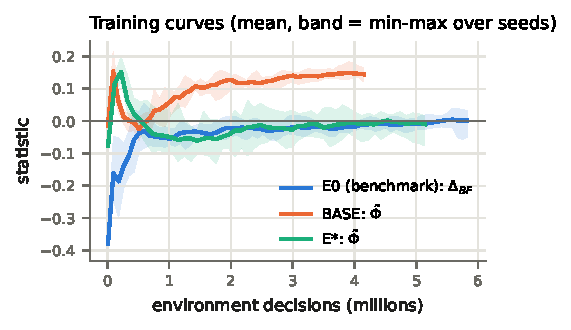
\includegraphics[width=\linewidth]{../figures/fig_curves.pdf}\caption{Learning curves: gap to the BF optimum
in E0, formateur premium $\tilde\Phi$ in the base game and E*.}\end{subfigure}\hfill
\begin{subfigure}[t]{0.29\textwidth}\centering
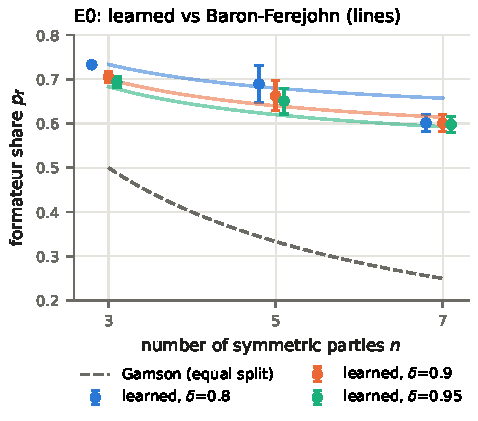
\includegraphics[width=\linewidth]{../figures/fig_e0_benchmark.pdf}\caption{E0: learned formateur share
(dots) vs the exact BF solution (lines).}\end{subfigure}\hfill
\begin{subfigure}[t]{0.345\textwidth}\centering
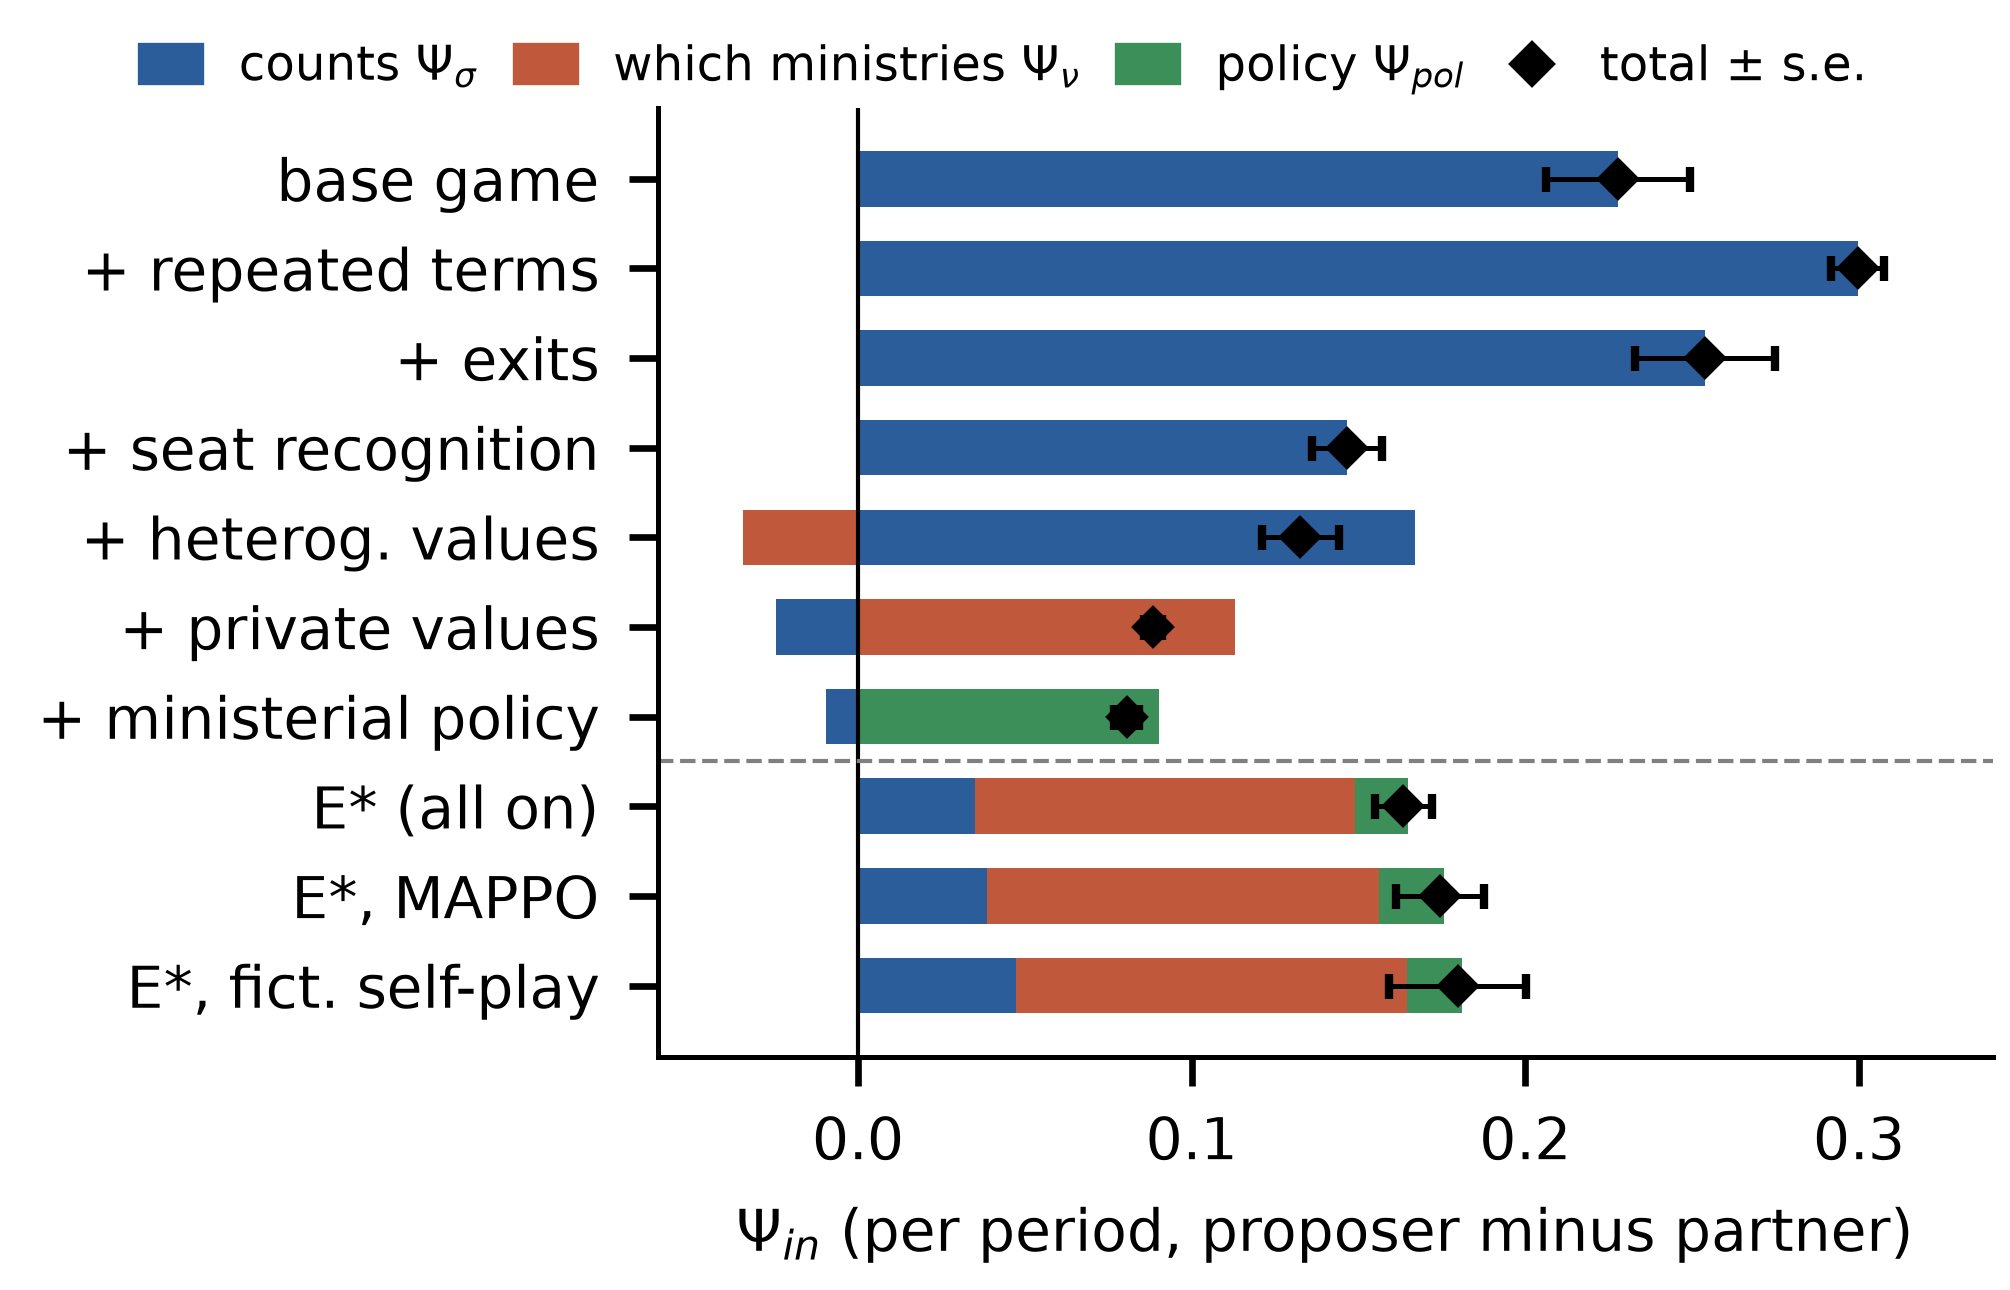
\includegraphics[width=\linewidth]{../figures/fig_psi.png}\caption{Value of proposal power $\Psi_{\mathrm{in}}$ by
reward channel (data: \texttt{results/psi\_summary.json}).}\end{subfigure}
\caption{Learning and results. (a) curves: mean over seeds, band min--max; (b), (c): 3--10 seeds.}
\label{fig:main}
\end{figure*}
After an election without a majority, parties bargain over who governs and how ministries are split.
Real coalition cabinets split ministries almost exactly in proportion to seats (\emph{Gamson's law}~\cite{gamson}).
The standard test regresses party $i$'s share of cabinet $c$'s ministries on its seat share in the coalition
and a formateur dummy,
\begin{equation}\label{eq:reg}
p_{ic}=\alpha+\beta\,s_{ic}+\gamma\,F_{ic}+\varepsilon_{ic};
\end{equation}
on \RealN{} real cabinets $\hat\alpha,\hat\beta,\hat\gamma=\RealA,\RealB,\RealG$ (prime minister's party as
$F$): proportional, no premium. Bargaining theory (Baron--Ferejohn, BF~\cite{bf}) predicts instead that the
\emph{formateur}, who proposes the cabinet, takes a large premium. Closed-form equilibria exist only for
toy versions; with indivisible ministries, policy, exits, repeated elections and private preferences the
game is unsolved. We therefore let \textbf{self-interested RL agents learn to bargain} and ask which rule
they arrive at. Everything is learned from environment rewards: no supervised targets, no search, no
fairness term. Scripted agents and exact solvers serve only as baselines and checks.

\section{RL formulation}
\paragraph{Environment} (\code{cabinet/env.py}). A partially observable stochastic game with $n$ parties
(seats $w_i$, majority quota $q$), $m$ ministries and an open-ended sequence of terms of $L$ periods. A
period without a cabinet is a \emph{formation round}: nature draws a formateur $f\sim\rho$, who proposes a
winning coalition $C\ni f$ and an assignment $\mu:\{1..m\}\to C$; it takes office only if every partner
accepts, otherwise a caretaker period passes. A period with a cabinet is a \emph{governance period}: each
member privately draws an exit bonus and stays or leaves; one exit collapses the cabinet. After each term
an election redraws seats and the episode continues with probability $\beta_T$. Institutional features
are switches added one at a time (\code{cabinet/config.py}): repeated terms (M1), demand bargaining (M2),
private types (M4), heterogeneous valuations (M5), exits (M8), ministerial policy (M9), seat-based
recognition (M10). Level E0 is the exact BF game; E* has every switch on ($n\le5$, $m=6$, $L=6$, 3 expected
terms, $\delta=0.9$).

\begin{table}[t]\centering\scriptsize\setlength{\tabcolsep}{2.5pt}
\caption{Observation of agent $i$ (\code{cabinet/env.py}, \texttt{observe}). Sets, not fixed vectors:
the size grows with $n$ and $m$; e.g.\ 323 numbers for $n=5$, $m=6$.}\label{tab:state}
\begin{tabular}{@{}l l >{\raggedright\arraybackslash}p{4.85cm}@{}}\toprule
part & shape & content \\\midrule
party tokens & $n\times26$ & seat share, recognition prob., self/formateur flags, membership and share in
proposal and cabinet, last votes and offers, policy distance (if public), last $\Lambda=4$ cabinets\\
ministry tokens & $m\times8$ & salience, own valuation, held by me, policy dimension led, own and current
policy\\
party--ministry & $m\times n\times4$ & others' valuations and policy cost (if public), who holds it\\
context & 17 & phase, time in term, quota, $\delta,\beta_T,\lambda,\xi,\bar e$, switches, $n,m$\\
decision & 8 & offer to me, its value, believed policy loss, bonus, \dots\\\bottomrule
\end{tabular}\end{table}

\paragraph{State space $\mathcal S$.} The full state holds seats, the clock, the proposal on the table,
the sitting cabinet, every party's type (valuations $\nu_i$ over ministries, ideal policy $z_i\in[0,1]^2$),
exit bonuses and recent history. Agents see only part of it (\cref{tab:state}): their own type, and others'
types only when types are public. Tokens carry no party labels, so one permutation-equivariant network
handles any $n,m$.

\begin{table}[t]\centering\scriptsize\setlength{\tabcolsep}{2.5pt}
\caption{Actions (all discrete). Proposals are built in $n{-}1{+}m$ masked steps instead of one choice
among up to 36{,}383 proposals (5 equal parties, 6 ministries).}\label{tab:action}
\begin{tabular}{@{}l l l@{}}\toprule
decision (who) & type & size \\\midrule
include party $j$? (formateur, by seats) & binary, masked & $n{-}1$ steps \\
ministry $k$ to whom? (formateur) & pointer over $C$ & $m$ steps of $\le|C|$ \\
offer to a partner (levels E0--E1) & 1\% grid & 101 \\
accept / reject (each partner) & binary & 2 \\
stay / exit (each member) & binary & 2 \\
demand or close (M2) & categorical & 102 \\\bottomrule
\end{tabular}\end{table}

\paragraph{Action space $\mathcal A$} (\cref{tab:action}). Masks make infeasible proposals impossible:
\emph{exclude} is blocked whenever the coalition could no longer win, and ministries go only to members.

\paragraph{Reward $\mathcal R$.} Each governed period, member $i$ of cabinet $(C,\mu)$ receives
\begin{equation}\label{eq:reward}
r_i=\underbrace{\textstyle\sum_{k:\mu(k)=i}\nu_{ik}}_{\text{office}}
-\underbrace{\lambda\tfrac1d\textstyle\sum_{h=1}^{d}|y_h-z_{ih}|}_{\text{policy loss}},
\end{equation}
where policy on dimension $h$ is the ideal point of the holder of its lead ministry,
$y_h=z_{\mu(\mathrm{lead}(h)),h}$ ($d=2$, $\lambda=0.5$); non-members get only the policy
term, a caretaker period gives no office, and an exiting member receives its bonus $e\sim0.05\,\mathrm{Exp}(1)$
once. Returns are discounted by $\delta$ per period. \emph{Incentive design}: rewards are individual and
contain no fairness or team term, so any proportionality must emerge; delay is costly through
discounting and caretaker periods; the policy term lets a party trade ministries for policy.

\paragraph{Algorithm} (\code{cabinet/policy.py}, \code{cabinet/ppo.py}). All parties share one policy
network (211k parameters): token MLPs, two attention blocks (self-attention over parties,
cross-attention to ministries), masked autoregressive heads (include/exclude, ministry pointer, offer,
vote, exit, demand) and a value head. Each agent acts only at some steps, so returns and GAE are computed
on its own decision sequence, accumulating discounted rewards between its decisions (a semi-MDP).
\textbf{Why PPO}~\cite{ppo}: the action space is structured and combinatorial with state-dependent masks,
which rules out tabular Q-learning and DQN's one output per action; PPO optimises the factorised
policy directly, its exact log-probability is the sum of masked steps, and clipped updates stay stable
while all agents learn simultaneously. Settings: 8192 decisions per iteration, 500--700 iterations
($\approx$5M decisions, 27\,min per E* run on a CPU), clip 0.2, GAE $\lambda=0.95$, entropy bonus
annealed $0.02\to0.002$ (5$\times$ on votes and exits), tuned on E0 only. Variants: MAPPO~\cite{mappo}
(critic on the global state), fictitious self-play and PSRO (\code{cabinet/psro.py}).

\paragraph{Baselines} (\code{cabinet/baselines.py}): BF agent (exact equilibrium, E0--E1), Gamson agent
(smallest winning coalition, split by seats), myopic BF heuristic, random feasible agent; the exact
solvers \code{cabinet/bf\_solver.py} and \code{cabinet/demand\_solver.py} validate learning.
\Cref{tab:base}: in E* the learned profile earns the most per seat and is the hardest to exploit.

\begin{table}[t]\centering\scriptsize\setlength{\tabcolsep}{3pt}
\caption{Baselines in E* (every party plays the profile; 3000 episodes). Payoff: per seat and period.
Exploit: what a PPO best response for one seat gains against the profile (lower is better). Formateur
coefficient $\hat\gamma$ of (1) in ministry counts.}\label{tab:base}
% learned: results/mech_Estar (10 seeds), results/exploit_Estar{,_br400}; scripted: evaluated on E*
% (cabinet.ppo.evaluate, 3000 episodes, seed 7) and results/baselines/seed0.json, exploit controls in
% results/exploit_Estar_br400/seed0.json
\begin{tabular}{@{}lcccc@{}}\toprule
profile & payoff & exploit & $\hat\gamma$ & failed rounds\\\midrule
PPO self-play (ours) & 0.15--0.16 & \GainLong & +0.052 & 0.05\\
Gamson agent & 0.122 & \GainLongGamson & $-0.001$ & 0.00\\
myopic BF heuristic & 0.096 & \GainLongMyopic & +0.274 & 0.25\\
random feasible & $-0.048$ & -- & $-0.006$ & 0.65\\\bottomrule
\end{tabular}\end{table}


\section{Results}
\paragraph{Learning is validated.} Training settles within 2--4M decisions (\cref{fig:main}a). In the BF
game the learned formateur share matches the exact solution (\cref{fig:main}b; mean absolute gap
\EzeroAbsGap, \EzeroCellsOK/9 cells within 0.02), including its fall with patience $\delta$. Outcomes
match equilibrium but play does not fully: learned voters would accept less than their reservation value
and formateurs never test it, so a best response gains up to \BrGainSeven{} per formation at $n=7$ (a
self-confirming pattern~\cite{fl}).

\paragraph{Proposal power pays; the premium changes currency.} The base game keeps a large premium
($\hat\gamma=\BaseGamma$). Private valuations ($\hat\gamma=\MfourGamma$) and ministerial policy
($\MnineGamma$) remove it \emph{in ministry counts}, yet the role still pays. Replaying saved states with each
coalition member forced to be the proposer (common random numbers), the same party earns more as proposer
than as partner: $\Psi_{\mathrm{in}}=\PsiMfour$, all in \emph{which} ministries it keeps
($\Psi_\nu=\PsiMfourNu$), with private values; \PsiMnine, all in policy, with ministerial policy; \PsiEstar{}
in E* (\cref{fig:main}c), with every learner.

\paragraph{Demand bargaining removes the premium but splits by voting weight.} On random 3--8-party
parliaments (pre-registered tests, 10 seeds per protocol), demands instead of proposals lower $\hat\gamma$
by \HoneDiff{} ($p=\HoneP$). Learned demand agents reproduce the exact equilibrium of the protocol: in a
45/35/20 parliament every pair splits 50/50 (within \AfDemMaxDev), where Gamson's law gives 0.56/0.44.

\paragraph{Real cabinets follow seats} (Seki--Williams~\cite{sw} with ParlGov~\cite{parlgov}; held out from
training). Partners with \emph{equal} voting weight still split by seats (slope \WvsSlope, \WvsPairs{} pairs),
and given the real coalition and prime minister, Gamson's law predicts real splits best (\cref{fig:real}:
error \MaeGamson{} per party vs \MaeBF{} for BF and \MaePrivLo--\MaePubHi{} for our agents).

\begin{figure}[t]\centering
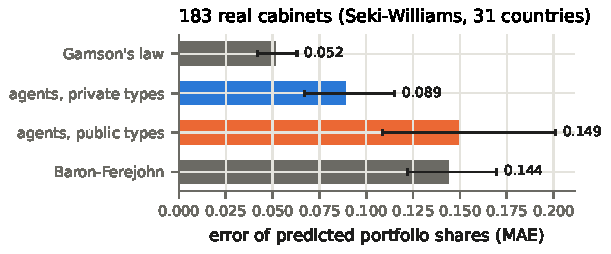
\includegraphics[width=0.92\columnwidth]{../figures/fig_real.pdf}
\caption{Predicting the ministry split of real coalition cabinets given the real coalition and prime
minister (mean absolute error per party; country-clustered 95\% CIs).}\label{fig:real}
\end{figure}

\section{Conclusion}
Self-interested RL parties favour the formateur exactly as far as the rules give it proposal power, and
otherwise split by voting weight; private information and policy move the premium out of ministry counts
rather than removing it. Real cabinets follow seats, so Gamson's law likely rests on rules outside these
models, such as commitments before the split~\cite{ks}. \textbf{Limitations}: scaled-down parliaments,
approximate equilibria (best responses gain \GainLongRel{} of a seat's payoff), and the prime minister's party
as a proxy for the formateur. Reproduction: \texttt{README.md}; every number: \code{docs/AUDIT.md}.

\begin{thebibliography}{9}\footnotesize\setlength{\itemsep}{0pt}
\bibitem{gamson} W. Gamson. A theory of coalition formation. \emph{Am. Sociol. Rev.} 26(3), 1961.
\bibitem{bf} D. Baron, J. Ferejohn. Bargaining in legislatures. \emph{APSR} 83(4), 1989.
\bibitem{ppo} J. Schulman et al. Proximal policy optimization algorithms. arXiv:1707.06347, 2017.
\bibitem{mappo} C. Yu et al. The surprising effectiveness of PPO in cooperative multi-agent games. NeurIPS, 2022.
\bibitem{fl} D. Fudenberg, D. Levine. Self-confirming equilibrium. \emph{Econometrica} 61(3), 1993.
\bibitem{sw} K. Seki, L. Williams. Updating the party government data set. \emph{Electoral Studies} 34, 2014.
\bibitem{parlgov} H. D\"oring, P. Manow. ParlGov: Parliaments and governments database. \url{https://www.parlgov.org}.
\bibitem{ks} A. Kamm, S. Siegenthaler. Commitment timing in coalitional bargaining. \emph{Exp. Econ.} 27, 2024.
\end{thebibliography}
\end{document}
